\documentclass{article}
\usepackage[a4paper,margin=1in]{geometry}
\usepackage{amsmath, amsfonts, amssymb, amstext, mathtools, stmaryrd, textcomp, xcolor, graphicx, tikz}
\usetikzlibrary{automata, positioning, arrows}
\tikzset{->,>=stealth,
every state/.style={thick, fill=gray!10}, 
initial text=$ $,
}
\newcommand{\e}{\varepsilon}
\newcommand{\s}{\Sigma}
\newcommand{\g}{\Gamma}
\newcommand{\so}{\rightarrow}
\newcommand{\str}{\texttt}
\newcommand{\newp}{\\[2mm]}
\newcommand{\defeq}{\coloneqq}

\title{Homework 02}
\author{Aaron Wang}
\date{January 31 2025}

\begin{document}
\maketitle
\begin{enumerate}
    \item \textbf{Divisibility tests.} Define, for all $k > 0$,
    \[
        D_k = \Big\{w \in \{\texttt{0}, . . . , \texttt{9}\}^*| w \text{ is the decimal representation of a multiple of } k \Big\}
    \]
    where $\e$ is considered to represent the number \texttt{0}. For example, the strings $\e$, \texttt{0}, \texttt{88}, and \texttt{088} all belong to $D_2$, but \texttt{99} and \texttt{099} do not.
    \begin{enumerate}
        \item Prove that $D_2$ is regular by writing a DFA for $D_2$.\newp
        
\textcolor{red}{
\begin{center}
\begin{minipage}{0.25\textwidth}
    i.
    \begin{center}
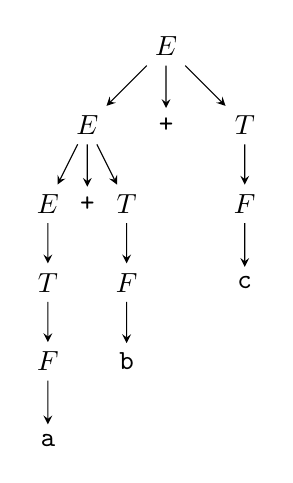
\begin{tikzpicture}[
    level distance=1cm,
    level 1/.style={sibling distance=1cm},
    level 2/.style={sibling distance=0.5cm}
]
    \node {$E$}
    child {node {$E$}
        child {node {$E$}
            child {node {$T$}
                child {node {$F$}
                    child {node {\str{a}}
                    }
                }
            }
        }
        child {node {\str{+}}}
        child {node {$T$}
            child {node {$F$}
                child {node {\str{b}}
                }
            }
        }
    }
    child {node {\str{+}}}
    child {node {$T$}
        child {node {$F$}
            child {node {\str{c}}}
        }
    };
\end{tikzpicture}
\end{center}
\end{minipage}
\begin{minipage}{0.25\textwidth}
    ii.
    \begin{center}
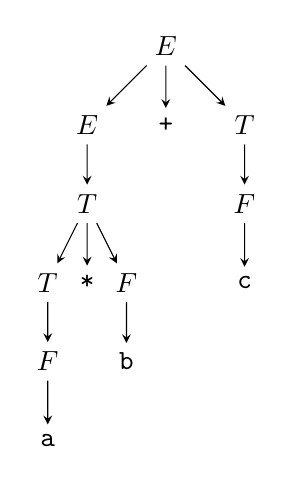
\begin{tikzpicture}[
    level distance=1cm,
    level 1/.style={sibling distance=1cm},
    level 2/.style={sibling distance=0.5cm}
]
    \node {$E$}
    child {node {$E$}
        child {node{$T$}
            child {node{$T$}
                child{node{$F$}
                    child{node{\str{a}}}
                }
            }
            child {node{\str{*}}}
            child {node{$F$}
                child{node {\str{b}}}
            }
        }
    }
    child {node {\str{+}}}
    child {node {$T$}
        child {node {$F$}
            child {node {\str{c}}}
        }
    };
\end{tikzpicture}
\end{center}
\end{minipage}
\begin{minipage}{0.25\textwidth}
    iii.
    \begin{center}
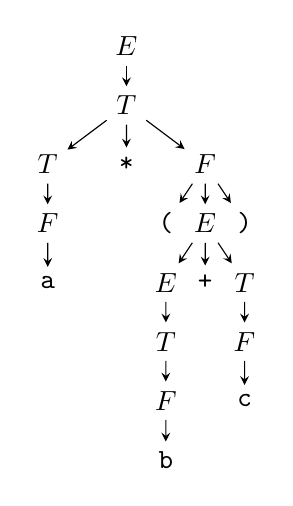
\begin{tikzpicture}[
    level distance=0.75cm,
    level 2/.style={sibling distance=1cm},
    level 3/.style={sibling distance=0.5cm}
]
    \node {$E$}
    child {node {$T$}
        child {node {$T$}
            child {node{$F$}
                child{node{\str{a}}}
            }
        }
        child {node {\str{*}}}
        child {node {$F$}
            child {node{\str{(}}}
            child {node {$E$}
                child {node {$E$}
                    child {node {$T$}
                        child {node{$F$}
                            child{node{\str{b}}}
                        }
                    }
                }
                child {node {\str{+}}}
                child {node {$T$}
                    child {node{$F$}
                        child{node{\str{c}}}
                    }
                }
            }
            child {node{\str{)}}}
        }
    };
\end{tikzpicture}
\end{center}
\end{minipage}
\end{center}
}

        \item Prove that $D_3$ is regular by writing a DFA for $D_3$.\newp
        \textcolor{red}{
\begin{align*}
& E \rightarrow E \: \str{+} \: T \: | \: T\\
& T \rightarrow T \: \str{*} \: F \: | \: F\\
& F \rightarrow O \: \str{$\uparrow$} \: F \: | \: O\\
& O \rightarrow \str{(}E\str{)} \: | \: \str{a} \: | \: \str{b} \: | \: \str{c}
\end{align*}
}
        \item Prove that $D_6$ is regular. An explicit DFA is not necessary.\newp
        \textcolor{red}{
    From the DFA of $D_2$ and $D_3$, we know that they are regular. Notice that for any number $w$, $w$ is a multiple of 6 if and only if $w$ is a multiple of 2 and 3. Thus, we can represent $D_6$ as:
    \[
        D_6 = \Big\{w \in \{\texttt{0}, . . . , \texttt{9}\}^*| w \text{ is the decimal representation of a multiple of } 2 \text{ and } 3 \Big\} = D_2 \cap D_3
    \]
    Thus $D_6$ is regular as it is the intersection of $D_2$ and $D_3$.\footnote{Theorem from class: If  $A$  and  $B$  are regular languages, then  $A \cap B$  is also regular.}
}

% skipped optional alternative
        % \item[(*)] Optional alternative: You can get full credit for all of the above if you can prove that for any $k > 0$, $D_k$ is regular, by describing how to write the formal description of a DFA $M = (Q, \{\texttt{0}, . . . , \texttt{9}\}, \delta, s, F)$ in terms of $k$.
    \end{enumerate}
    \item \textbf{Nondeterminism.} Consider the following NFA $N_2$ (same as in Figure 1.31), which accepts a string iff the third-to-last symbol is a 1:
    \item[1.] $z^3$
\begin{align*}
    u(x,y) &= x^3 - 3xy^2\\
    v(x,y) &= 3xy^2 - y^3
\end{align*}
\begin{align*}
    \pd{u}{x}  &= 3x^2 - 3y^2  &\qquad \pd{v}{y}  &= 3x^2 - 3y^2 \\
    \pd{u}{y} &= -6xy           &\qquad \pd{v}{x} &= 6xy
\end{align*}

\answer{
Since $\pd{u}{x} = \pd{v}{y}$ and $-\pd{u}{y} = \pd{v}{x}$, $f(z) = z^3$ is analytical.
}

    \begin{enumerate}
        \item Use the subset construction (Theorem 1.39) to convert $N_2$ to a DFA $M$. You may omit curly braces and commas when naming states; for example, instead of $\{1, 2, 3, 4\}$ you may write 1234. (Hint: the DFA should be equivalent to the one in Figure 1.32.)
        \begin{figure}[h]
\centering
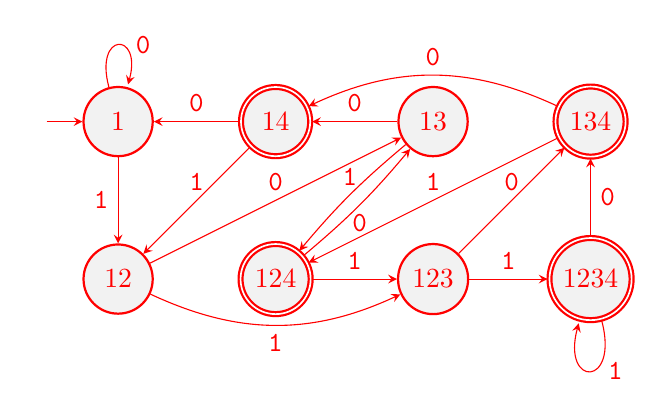
\begin{tikzpicture}
\color{red}
    % \node[state, initial] (q000) {$q_{000}$};
    % \node[state, yshift=-2cm] (q001) {$q_{001}$};
    % \node[state, xshift=4cm] (q010) {$q_{010}$};
    % \node[state, yshift=-2cm, xshift=4cm] (q011) {$q_{011}$};
    % \node[state, xshift=2cm, accepting] (q100) {$q_{100}$};
    % \node[state, yshift=-2cm, xshift=2cm, accepting] (q101) {$q_{101}$};
    % \node[state, xshift=6cm, accepting] (q110) {$q_{110}$};
    % \node[state, yshift=-2cm, xshift=6cm, accepting] (q111) {$q_{111}$};
    \node[state, initial] (q000) {1};
    \node[state, yshift=-2cm] (q001) {12};
    \node[state, xshift=4cm] (q010) {13};
    \node[state, yshift=-2cm, xshift=4cm] (q011) {123};
    \node[state, xshift=2cm, accepting] (q100) {14};
    \node[state, yshift=-2cm, xshift=2cm, accepting] (q101) {124};
    \node[state, xshift=6cm, accepting] (q110) {134};
    \node[state, yshift=-2cm, xshift=6cm, accepting] (q111) {1234};
    \draw 
        (q000) edge[loop above] node[right, xshift=1mm]{\str{0}} (q000)
        (q000) edge[] node[left]{\str{1}} (q001)
        (q001) edge[] node[above]{\str{0}} (q010)
        (q001) edge[bend right=25] node[below]{\str{1}} (q011)
        (q100) edge[] node[above]{\str{0}} (q000)
        (q100) edge[] node[above]{\str{1}} (q001)
        (q101) edge[bend right=5] node[below]{\str{0}} (q010)
        (q101) edge[] node[above]{\str{1}} (q011)
        (q010) edge[] node[above]{\str{0}} (q100)
        (q010) edge[bend right=5] node[above]{\str{1}} (q101)
        (q011) edge[] node[above]{\str{0}} (q110)
        (q011) edge[] node[above]{\str{1}} (q111)
        (q110) edge[bend right=25] node[above]{\str{0}} (q100)
        (q110) edge[] node[above]{\str{1}} (q101)
        (q111) edge[] node[right]{\str{0}} (q110)
        (q111) edge[loop below] node[right, xshift=1mm]{\str{1}} (q111)
    ;
\end{tikzpicture}
\end{figure}
        \item  Why are the states in Figure 1.32 named $q_{abc}$ where $a, b, c \in\{\texttt{0}, \texttt{1}\}$?\newp
        \textcolor{red}{
    Proof: Assume $ADD$ is a regular language. Let $p$ be the pumping length from the Pumping Lemma. Let $s = \str{1}^p\str{=1}^p\str{+0}$. Observe that $s \in ADD$. The Pumping Lemma says that for some $xyz$, $s=xyz$, $|y| > 0$, $|xy| \leq p$ and $xyyz \in ADD$. Let $s' = xyyz$. Since $|xy| \leq p$, we know that $y$ contains all \str{1}s so $s' = \str{1}^r\str{=1}^p\str{+0}$ s.t. $r > p$. $s'$ is not true as  a number + 0 should be itself but it is not in this expression. Since $s'$ is not a true expression, $s' \notin ADD$ $\lightning$. Thus, by contradiction we have shown that $ADD$ can not be a regular language.
}
        \item In Example 1.30, Sipser asks what happens if you modify $N_2$ into the following NFA - let’s call it $N'_2$:
        \item $x\sqrt{1-y^2}dx+y\sqrt{1-x^2}dy=0$, $y = \frac{1}{2}$ when $x = \frac{1}{2}$
    
    \textcolor{blue}{
    \begin{minipage}[t]{0.45\textwidth}
        General Solution:
        \begin{gather*}
            x\sqrt{1-y^2}dx+y\sqrt{1-x^2}dy = 0 \\
            y\sqrt{1-x^2}dy = -x\sqrt{1-y^2}dx \\
            \frac{y}{\sqrt{1-y^2}}dy = -\frac{x}{\sqrt{1-x^2}}dx \\
            \int\frac{y}{\sqrt{1-y^2}}dy = -\int\frac{x}{\sqrt{1-x^2}}dx \\
            -\frac{1}{2}\sqrt{1-y^2} = \frac{1}{2}\sqrt{1-x^2}+C \\
            \frac{1}{2}\sqrt{1-y^2} + \frac{1}{2}\sqrt{1-x^2} = C \\
            \textcolor{red}{
            \sqrt{1-y^2} + \sqrt{1-x^2} = C   
            }
        \end{gather*}
    \end{minipage}
    \hfill
    \begin{minipage}[t]{0.45\textwidth}
        Integration:\\
            $u = 1-t^2$; $du = -2tdt$; $dt = -\frac{1}{2t}du$      
        \[
            \int\frac{t}{\sqrt{1-t^2}}dt =\int\frac{t}{\sqrt{u}}\frac{-1}{2t}du
        \]
        \[
            =-\frac{1}{2}\int\frac{1}{\sqrt{u}}du
            = -\frac{1}{2}(\sqrt{u})+C
        \]
        \[= -\frac{1}{2}\sqrt{1-t^2}+C\]
        Particular Solution:
        \begin{gather*}
            \sqrt{1-(1/2)^2} + \sqrt{1-(1/2)^2} = C \\
            C = \sqrt{3/4}+\sqrt{3/4} = \sqrt3 \\
            \textcolor{red}{
            \sqrt{1-y^2} + \sqrt{1-x^2} = \sqrt3
            }
        \end{gather*}
    \end{minipage}
    }\newp
        \textcolor{red}{
    This now accepts the string if \str{1} is the last, second-to-last, or third-to-last character.
}
        \item Use the subset construction (Theorem 1.39) to convert $N'_2$ to a DFA $M'$.
        \begin{figure}[!h]
\centering
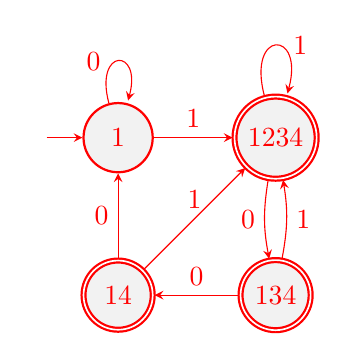
\begin{tikzpicture}
\color{red}
    % \node[state, initial] (q000) {$q_{000}$};
    % \node[state, yshift=-2cm, accepting] (q001) {$q_{001}$};
    % \node[state, xshift=4cm, accepting] (q010) {$q_{010}$};
    % \node[state, yshift=-2cm, xshift=4cm, accepting] (q011) {$q_{011}$};
    % \node[state, xshift=2cm, accepting] (q100) {$q_{100}$};
    % \node[state, yshift=-2cm, xshift=2cm, accepting] (q101) {$q_{101}$};
    % \node[state, xshift=6cm, accepting] (q110) {$q_{110}$};
    % \node[state, yshift=-2cm, xshift=6cm, accepting] (q111) {$q_{111}$};
    % \draw 
    %     (q000) edge[loop above] node[right, xshift=1mm]{\str{0}} (q000)
    %     (q000) edge[] node[left]{\str{1}} (q001)
    %     (q001) edge[] node[above]{\str{0}} (q010)
    %     (q001) edge[bend right=25] node[below]{\str{1}} (q011)
    %     (q100) edge[] node[above]{\str{0}} (q000)
    %     (q100) edge[] node[above]{\str{1}} (q001)
    %     (q101) edge[bend right=5] node[below]{\str{0}} (q010)
    %     (q101) edge[] node[above]{\str{1}} (q011)
    %     (q010) edge[] node[above]{\str{0}} (q100)
    %     (q010) edge[bend right=5] node[above]{\str{1}} (q101)
    %     (q011) edge[] node[above]{\str{0}} (q110)
    %     (q011) edge[] node[above]{\str{1}} (q111)
    %     (q110) edge[bend right=25] node[above]{\str{0}} (q100)
    %     (q110) edge[] node[above]{\str{1}} (q101)
    %     (q111) edge[] node[right]{\str{0}} (q110)
    %     (q111) edge[loop right] node[above, yshift=1mm]{\str{1}} (q111)
    % ;
    \node[state, initial] (q1) {1};
    \node[state, xshift=2cm, accepting] (q2) {1234};
    \node[state, xshift=2cm, yshift=-2cm, accepting] (q3) {134};
    \node[state, yshift=-2cm, accepting] (q4) {14};
    \draw
        (q1) edge[loop above] node[left, xshift=-1mm]{0} (q1)
        (q1) edge[] node[above]{1} (q2)
        (q2) edge[loop above] node[right, xshift=1mm]{1} (q2)
        (q2) edge[bend right=10] node[left]{0} (q3)
        (q3) edge[bend right=10] node[right]{1} (q2)
        (q3) edge[] node[above]{0} (q4)
        (q4) edge[] node[left]{0} (q1)
        (q4) edge[] node[above]{1} (q2)
        ;
\end{tikzpicture}
\end{figure}
    \end{enumerate}
\newpage
    \item \textbf{Procrustean closure properties.} Let $\s$ be an alphabet, and let $L_3 = \{\texttt{theory}, \texttt{of}, \texttt{computing}\}$ be an example language.
    \begin{enumerate}
%3a%
        \item For any $w = w_1w_2 \cdots w_{n-1}w_n$, define
        \[
        \text{STRETCH}(w_1w_2 \cdots w_n) = w_1w_1w_2w_2 \cdots w_{n-1}w_{n-1}w_nw_n. 
        \]
        This induces an operation on languages,
        \[
        \text{STRETCH}(L) = \{\text{STRETCH}(w) | w \in L\}.  
        \]
        For example,
        \[
        \text{STRETCH}(L_3) = \{\texttt{tthheeoorryy}, \texttt{ooff}, \texttt{ccoommppuuttiinngg}\}.
        \]
        Prove that if $L$ is a regular language, then STRETCH$(L)$ is also regular.\newp
        \textcolor{red}{
    If $L$ is regular, we have an NFA without $\e$ transitions $N$ for $L$ s.t. $N = (Q, \s, \delta, s, F)$.\\
    Construct $N'= (Q', \s, \delta', s, F)$ to recognize STRETCH$(L)$\\
    \begin{enumerate}
        \item [1.]$Q'= Q \cup (\s_\e \times Q)$. This way we have the regular states and a state for every transition.
        \item [2.] $\s$ does not change.
        \item [3.] Define $\delta'$ so if $q$ is an original state ($q \in Q$), it will give transition state(s) and vice versa.
        \[
        \delta'\Big(q,a\Big)=  
        \begin{cases}
         (a,\delta(q,a)) & q \in Q  \\
         q_{\text{next(s)}}  & \text{s.t. } (a,q_{\text{next(s)}}) = q\\
         \emptyset & \text{otherwise}
        \end{cases}
        \]
        \item [4.] $s$ does not change.
        \item [5.] $F$ does not change.
    \end{enumerate}
    Let $L=\{\str{in},\str{out}\}$ as an example.\footnote{States without transitions were ommited from drawing}\\
    \begin{figure}[h]
\centering
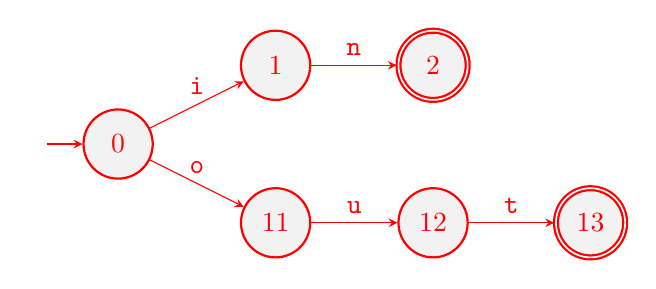
\begin{tikzpicture}
\color{red}
    \node[state, initial] (q0) {0};
    \node[state, xshift=2cm, yshift=1cm] (q1) {1};
    \node[state, xshift=4cm, yshift=1cm, accepting] (q2) {2};
    \node[state, xshift=2cm, yshift=-1cm] (q11) {11};
    \node[state, xshift=4cm, yshift=-1cm] (q12) {12};
    \node[state, xshift=6cm, yshift=-1cm, accepting] (q13) {13};
    
    \draw
    (q0) edge[] node[above]{\str{i}} (q1)
    (q1) edge[] node[above]{\str{n}} (q2)

    (q0) edge[] node[above]{\str{o}} (q11)
    (q11) edge[] node[above]{\str{u}} (q12)
    (q12) edge[] node[above]{\str{t}} (q13)
    ;
\end{tikzpicture}
\end{figure}\\
    STRETCH$(L)$
    \begin{figure}[h]
\centering
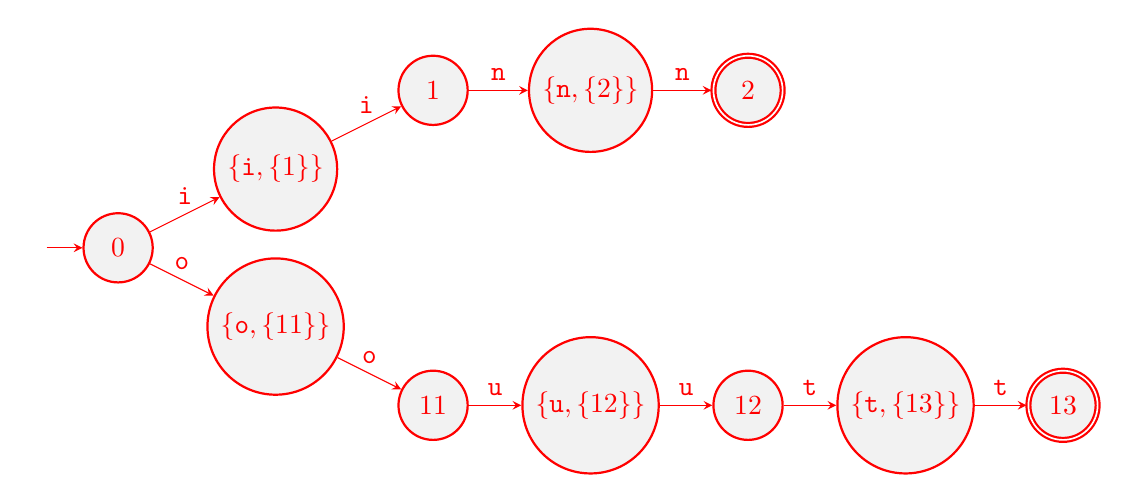
\begin{tikzpicture}
\color{red}
    \node[state, initial] (q0) {0};
    \node[state, xshift=2cm, yshift=1cm] (q1) {$\{\str{i},\{1\}\}$};
    \node[state, xshift=4cm, yshift=2cm] (q2) {1};
    \node[state, xshift=6cm, yshift=2cm] (q3) {$\{\str{n},\{2\}\}$};
    \node[state, xshift=8cm, yshift=2cm, accepting] (q4) {2};
    
    \node[state, xshift=2cm, yshift=-1cm] (q11) {$\{\str{o},\{11\}\}$};
    \node[state, xshift=4cm, yshift=-2cm] (q12) {11};
    \node[state, xshift=6cm, yshift=-2cm] (q13) {$\{\str{u},\{12\}\}$};
    \node[state, xshift=8cm, yshift=-2cm] (q14) {12};
    \node[state, xshift=10cm, yshift=-2cm] (q15) {$\{\str{t},\{13\}\}$};
    \node[state, xshift=12cm, yshift=-2cm, accepting] (q16) {13};
    
    \draw
    (q0) edge[] node[above]{\str{i}} (q1)
    (q1) edge[] node[above]{\str{i}} (q2)
    (q2) edge[] node[above]{\str{n}} (q3)
    (q3) edge[] node[above]{\str{n}} (q4)

    (q0) edge[] node[above]{\str{o}} (q11)
    (q11) edge[] node[above]{\str{o}} (q12)
    (q12) edge[] node[above]{\str{u}} (q13)
    (q13) edge[] node[above]{\str{u}} (q14)
    (q14) edge[] node[above]{\str{t}} (q15)
    (q15) edge[] node[above]{\str{t}} (q16)
    ;
\end{tikzpicture}
\end{figure}\\
    By proof of construction STRETCH$(L)$ is regular.
}
\newpage
%3b%
        \item For any $w = w_1w_2\cdots w_{n-1}w_n$ with $n \geq 2$, define 
        \[\text{CHOP}(w_1w_2\cdots w_{n-1}w_n) = w_2\cdots w_{n-1}.\] 
        This induces an operation on languages,
        \[\text{CHOP} = \{\text{CHOP}(w) | w \in L \text{ and } |w| \geq 2\}.\]
        For example,
        \[
            \text{CHOP}(L_3) = \{\texttt{heor}, \e, \texttt{omputin}\}.
        \]
        Prove that if $L$ is a regular language, then CHOP$(L)$ is also regular.\newp
        \textcolor{red}{
    Proof: Assume $C$ is a regular language. Let $p$ be the pumping length from the Pumping Lemma. Let $s = \str{1}^p\str{01}^p$. Observe that $s \in C$. The Pumping Lemma says that for some $xyz$, $s=xyz$, $|y| > 0$, $|xy| \leq p$ and $xz \in C$. Let $s' = xz$. Since $|xy| \leq p$, we know that $y$ contains all \str{1}s so $s' = \str{1}^r\str{01}^p$ s.t. $r < p$. Thus $k \leq r$ and $w$ contains more than $p-1=r$ \str{1}s so $s' \notin L$ $\lightning$. Thus, by contradiction we have shown that $C$ can not be a regular language.
}
    \end{enumerate}
\end{enumerate}
\end{document}